%{\color{gray}\hrule}
%\usepackage{graphicx}
\begin{minipage}[t]{0.6\textwidth}
    \section{Datasets}
    Various Datasets were tested with, namely : 
    \begin{itemize}
        \item MNIST Handwritten Digits Dataset
        \item EMNIST
        \item USPS
        \item SVHN
    \end{itemize}
    But all these datasets had a problem that the models trained on them don't translate well into detecting digits on a Sudoku grid as there's a lot of noise in each of the extracted cells or boxes as seen in Figure.1.
    \begin{center}
        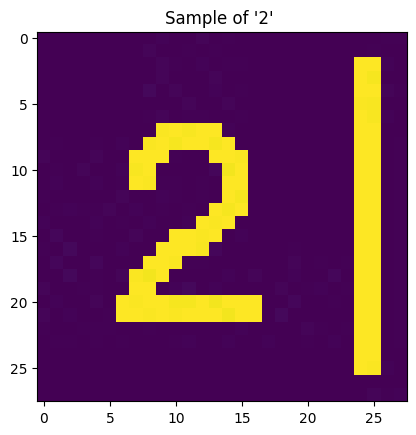
\includegraphics[width=2in]{2.png}
        \captionof{figure}{A sample of image '2'}
        \label{fig:figure_label}
    \end{center}
    Due to such noise the accuracy of these models in recognizing the Sudoku Digits decreases which is the most essential part of the models performance. The models performance on the training data can be good, but after testing on real sudoku images the model's performace was subpar.
    So 'Printed Digit Dataset' was used.It Contains around 3000 images of digitally printed numeric dataset.
    Each image is of dimension 28x28 and is grayscale. This dataset was purposely created for sudoku digits classification hence it shows blank image for 0 (zeros).

\end{minipage}




